\documentclass{extbook}[14pt]
\usepackage{multicol, enumerate, enumitem, hyperref, color, soul, setspace, parskip, fancyhdr, amssymb, amsthm, amsmath, latexsym, units, mathtools}
\everymath{\displaystyle}
\usepackage[headsep=0.5cm,headheight=0cm, left=1 in,right= 1 in,top= 1 in,bottom= 1 in]{geometry}
\usepackage{dashrule}  % Package to use the command below to create lines between items
\newcommand{\litem}[1]{\item #1

\rule{\textwidth}{0.4pt}}
\pagestyle{fancy}
\lhead{}
\chead{Answer Key for Progress Quiz 6 Version C}
\rhead{}
\lfoot{9689-6866}
\cfoot{}
\rfoot{Spring 2021}
\begin{document}
\textbf{This key should allow you to understand why you choose the option you did (beyond just getting a question right or wrong). \href{https://xronos.clas.ufl.edu/mac1105spring2020/courseDescriptionAndMisc/Exams/LearningFromResults}{More instructions on how to use this key can be found here}.}

\textbf{If you have a suggestion to make the keys better, \href{https://forms.gle/CZkbZmPbC9XALEE88}{please fill out the short survey here}.}

\textit{Note: This key is auto-generated and may contain issues and/or errors. The keys are reviewed after each exam to ensure grading is done accurately. If there are issues (like duplicate options), they are noted in the offline gradebook. The keys are a work-in-progress to give students as many resources to improve as possible.}

\rule{\textwidth}{0.4pt}

\begin{enumerate}\litem{
Construct the lowest-degree polynomial given the zeros below. Then, choose the intervals that contain the coefficients of the polynomial in the form $ax^3+bx^2+cx+d$.
\[ \frac{-2}{5}, -6, \text{ and } \frac{4}{3} \]The solution is \( 15x^{3} +76 x^{2} -92 x -48 \), which is option B.\begin{enumerate}[label=\Alph*.]
\item \( a \in [12, 19], b \in [72, 81], c \in [-96, -91], \text{ and } d \in [47, 50] \)

$15x^{3} +76 x^{2} -92 x + 48$, which corresponds to multiplying everything correctly except the constant term.
\item \( a \in [12, 19], b \in [72, 81], c \in [-96, -91], \text{ and } d \in [-54, -45] \)

* $15x^{3} +76 x^{2} -92 x -48$, which is the correct option.
\item \( a \in [12, 19], b \in [58, 66], c \in [-152, -146], \text{ and } d \in [47, 50] \)

$15x^{3} +64 x^{2} -148 x + 48$, which corresponds to multiplying out $(5x -2)(x + 6)(3x -4)$.
\item \( a \in [12, 19], b \in [-79, -73], c \in [-96, -91], \text{ and } d \in [47, 50] \)

$15x^{3} -76 x^{2} -92 x + 48$, which corresponds to multiplying out $(5x -2)(x -6)(3x + 4)$.
\item \( a \in [12, 19], b \in [-124, -115], c \in [159, 171], \text{ and } d \in [-54, -45] \)

$15x^{3} -116 x^{2} +164 x -48$, which corresponds to multiplying out $(5x -2)(x -6)(3x -4)$.
\end{enumerate}

\textbf{General Comment:} To construct the lowest-degree polynomial, you want to multiply out $(5x + 2)(x + 6)(3x -4)$
}
\litem{
Describe the zero behavior of the zero $x = 4$ of the polynomial below.
\[ f(x) = -6(x + 3)^{11}(x - 3)^{7}(x + 4)^{9}(x - 4)^{4} \]The solution is the graph below, which is option B.
\begin{center}
    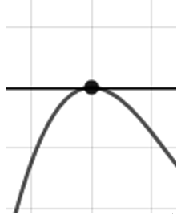
\includegraphics[width=0.3\textwidth]{../Figures/polyZeroBehaviorBC.png}
\end{center}\begin{enumerate}[label=\Alph*.]
\begin{multicols}{2}
\item 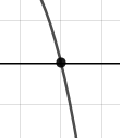
\includegraphics[width = 0.3\textwidth]{../Figures/polyZeroBehaviorAC.png}
\item 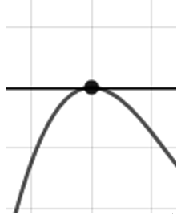
\includegraphics[width = 0.3\textwidth]{../Figures/polyZeroBehaviorBC.png}
\item 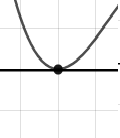
\includegraphics[width = 0.3\textwidth]{../Figures/polyZeroBehaviorCC.png}
\item 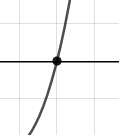
\includegraphics[width = 0.3\textwidth]{../Figures/polyZeroBehaviorDC.png}
\end{multicols}\item None of the above.\end{enumerate}
\textbf{General Comment:} You will need to sketch the entire graph, then zoom in on the zero the question asks about.
}
\litem{
Which of the following equations \textit{could} be of the graph presented below?

\begin{center}
    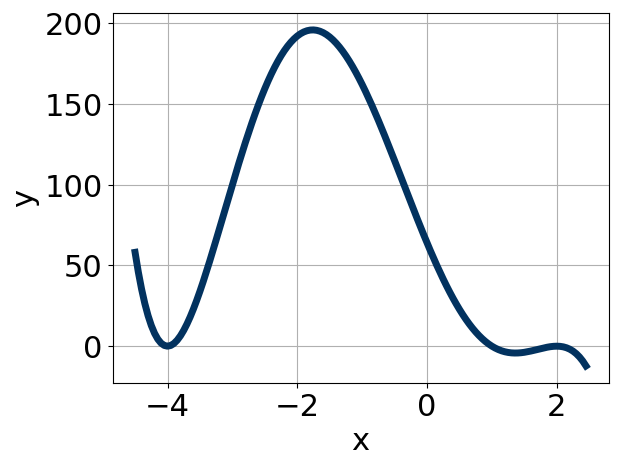
\includegraphics[width=0.5\textwidth]{../Figures/polyGraphToFunctionC.png}
\end{center}


The solution is \( -18x^{5} (x + 2)^{8} (x - 2)^{8} \), which is option C.\begin{enumerate}[label=\Alph*.]
\item \( 11x^{11} (x + 2)^{6} (x - 2)^{4} \)

This corresponds to the leading coefficient being the opposite value than it should be.
\item \( -7x^{9} (x + 2)^{4} (x - 2)^{9} \)

The factor $(x - 2)$ should have an even power.
\item \( -18x^{5} (x + 2)^{8} (x - 2)^{8} \)

* This is the correct option.
\item \( 17x^{10} (x + 2)^{6} (x - 2)^{6} \)

The factor $x$ should have an odd power and the leading coefficient should be the opposite sign.
\item \( -12x^{6} (x + 2)^{10} (x - 2)^{7} \)

The factor $(x - 2)$ should have an even power and the factor $x$ should have an odd power.
\end{enumerate}

\textbf{General Comment:} General Comments: Draw the x-axis to determine which zeros are touching (and so have even multiplicity) or cross (and have odd multiplicity).
}
\litem{
Describe the zero behavior of the zero $x = -3$ of the polynomial below.
\[ f(x) = -6(x - 3)^{8}(x + 3)^{9}(x + 9)^{3}(x - 9)^{5} \]The solution is the graph below, which is option D.
\begin{center}
    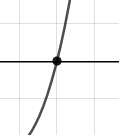
\includegraphics[width=0.3\textwidth]{../Figures/polyZeroBehaviorCopyDC.png}
\end{center}\begin{enumerate}[label=\Alph*.]
\begin{multicols}{2}
\item 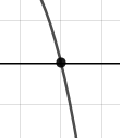
\includegraphics[width = 0.3\textwidth]{../Figures/polyZeroBehaviorCopyAC.png}
\item 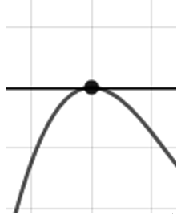
\includegraphics[width = 0.3\textwidth]{../Figures/polyZeroBehaviorCopyBC.png}
\item 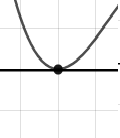
\includegraphics[width = 0.3\textwidth]{../Figures/polyZeroBehaviorCopyCC.png}
\item 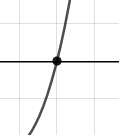
\includegraphics[width = 0.3\textwidth]{../Figures/polyZeroBehaviorCopyDC.png}
\end{multicols}\item None of the above.\end{enumerate}
\textbf{General Comment:} You will need to sketch the entire graph, then zoom in on the zero the question asks about.
}
\litem{
Which of the following equations \textit{could} be of the graph presented below?

\begin{center}
    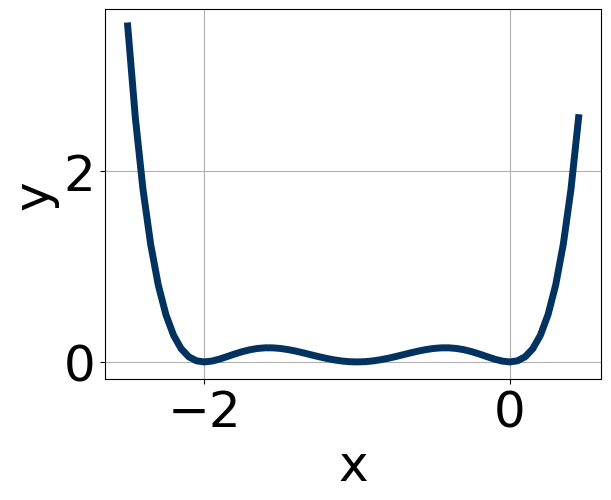
\includegraphics[width=0.5\textwidth]{../Figures/polyGraphToFunctionCopyC.png}
\end{center}


The solution is \( -19(x + 3)^{8} (x + 4)^{10} (x + 2)^{6} \), which is option B.\begin{enumerate}[label=\Alph*.]
\item \( -4(x + 3)^{8} (x + 4)^{11} (x + 2)^{11} \)

The factors $(x + 4)$ and $(x + 2)$ should both have even powers.
\item \( -19(x + 3)^{8} (x + 4)^{10} (x + 2)^{6} \)

* This is the correct option.
\item \( -4(x + 3)^{4} (x + 4)^{8} (x + 2)^{9} \)

The factor $(x + 2)$ should have an even power.
\item \( 18(x + 3)^{10} (x + 4)^{6} (x + 2)^{6} \)

This corresponds to the leading coefficient being the opposite value than it should be.
\item \( 2(x + 3)^{4} (x + 4)^{4} (x + 2)^{11} \)

The factor $(x + 2)$ should have an even power and the leading coefficient should be the opposite sign.
\end{enumerate}

\textbf{General Comment:} General Comments: Draw the x-axis to determine which zeros are touching (and so have even multiplicity) or cross (and have odd multiplicity).
}
\litem{
Describe the end behavior of the polynomial below.
\[ f(x) = 3(x - 2)^{3}(x + 2)^{6}(x - 3)^{3}(x + 3)^{5} \]The solution is the graph below, which is option D.
\begin{center}
    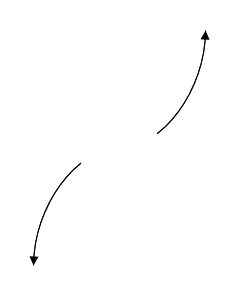
\includegraphics[width=0.3\textwidth]{../Figures/polyEndBehaviorCopyDC.png}
\end{center}\begin{enumerate}[label=\Alph*.]
\begin{multicols}{2}
\item 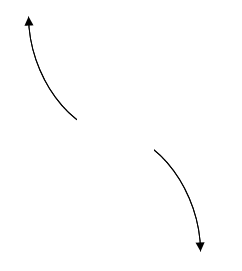
\includegraphics[width = 0.3\textwidth]{../Figures/polyEndBehaviorCopyAC.png}
\item 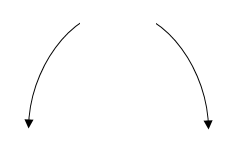
\includegraphics[width = 0.3\textwidth]{../Figures/polyEndBehaviorCopyBC.png}
\item 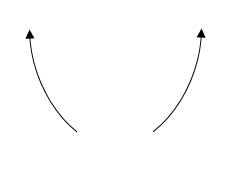
\includegraphics[width = 0.3\textwidth]{../Figures/polyEndBehaviorCopyCC.png}
\item 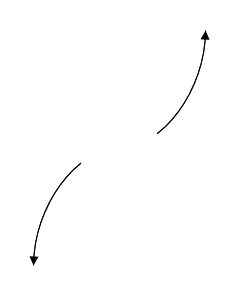
\includegraphics[width = 0.3\textwidth]{../Figures/polyEndBehaviorCopyDC.png}
\end{multicols}\item None of the above.\end{enumerate}
\textbf{General Comment:} Remember that end behavior is determined by the leading coefficient AND whether the \textbf{sum} of the multiplicities is positive or negative.
}
\litem{
Construct the lowest-degree polynomial given the zeros below. Then, choose the intervals that contain the coefficients of the polynomial in the form $x^3+bx^2+cx+d$.
\[ 4 + 5 i \text{ and } -2 \]The solution is \( x^{3} -6 x^{2} +25 x + 82 \), which is option A.\begin{enumerate}[label=\Alph*.]
\item \( b \in [-7, 0], c \in [24.91, 26.45], \text{ and } d \in [80.64, 83.45] \)

* $x^{3} -6 x^{2} +25 x + 82$, which is the correct option.
\item \( b \in [-1, 2], c \in [-3.56, -2.79], \text{ and } d \in [-10.45, -8.73] \)

$x^{3} + x^{2} -3 x -10$, which corresponds to multiplying out $(x -5)(x + 2)$.
\item \( b \in [2, 10], c \in [24.91, 26.45], \text{ and } d \in [-84.05, -81.44] \)

$x^{3} +6 x^{2} +25 x -82$, which corresponds to multiplying out $(x-(4 + 5 i))(x-(4 - 5 i))(x -2)$.
\item \( b \in [-1, 2], c \in [-2.86, -1.28], \text{ and } d \in [-9.04, -7.02] \)

$x^{3} + x^{2} -2 x -8$, which corresponds to multiplying out $(x -4)(x + 2)$.
\item \( \text{None of the above.} \)

This corresponds to making an unanticipated error or not understanding how to use nonreal complex numbers to create the lowest-degree polynomial. If you chose this and are not sure what you did wrong, please contact the coordinator for help.
\end{enumerate}

\textbf{General Comment:} Remember that the conjugate of $a+bi$ is $a-bi$. Since these zeros always come in pairs, we need to multiply out $(x-(4 + 5 i))(x-(4 - 5 i))(x-(-2))$.
}
\litem{
Describe the end behavior of the polynomial below.
\[ f(x) = -4(x + 2)^{3}(x - 2)^{4}(x - 7)^{4}(x + 7)^{6} \]The solution is the graph below, which is option A.
\begin{center}
    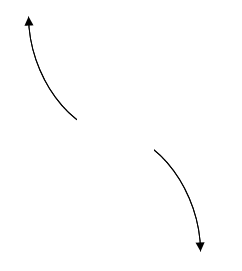
\includegraphics[width=0.3\textwidth]{../Figures/polyEndBehaviorAC.png}
\end{center}\begin{enumerate}[label=\Alph*.]
\begin{multicols}{2}
\item 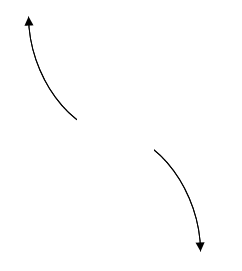
\includegraphics[width = 0.3\textwidth]{../Figures/polyEndBehaviorAC.png}
\item 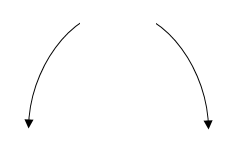
\includegraphics[width = 0.3\textwidth]{../Figures/polyEndBehaviorBC.png}
\item 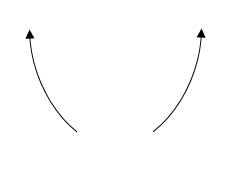
\includegraphics[width = 0.3\textwidth]{../Figures/polyEndBehaviorCC.png}
\item 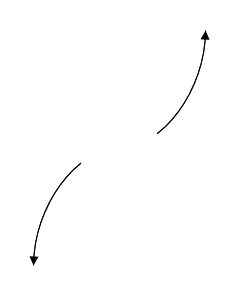
\includegraphics[width = 0.3\textwidth]{../Figures/polyEndBehaviorDC.png}
\end{multicols}\item None of the above.\end{enumerate}
\textbf{General Comment:} Remember that end behavior is determined by the leading coefficient AND whether the \textbf{sum} of the multiplicities is positive or negative.
}
\litem{
Construct the lowest-degree polynomial given the zeros below. Then, choose the intervals that contain the coefficients of the polynomial in the form $x^3+bx^2+cx+d$.
\[ 4 + 2 i \text{ and } -4 \]The solution is \( x^{3} -4 x^{2} -12 x + 80 \), which is option A.\begin{enumerate}[label=\Alph*.]
\item \( b \in [-4.2, -2.5], c \in [-14.9, -10.4], \text{ and } d \in [75, 81] \)

* $x^{3} -4 x^{2} -12 x + 80$, which is the correct option.
\item \( b \in [-1.7, 2.1], c \in [0.3, 5.3], \text{ and } d \in [-10, -2] \)

$x^{3} + x^{2} +2 x -8$, which corresponds to multiplying out $(x -2)(x + 4)$.
\item \( b \in [2.9, 6.9], c \in [-14.9, -10.4], \text{ and } d \in [-82, -79] \)

$x^{3} +4 x^{2} -12 x -80$, which corresponds to multiplying out $(x-(4 + 2 i))(x-(4 - 2 i))(x -4)$.
\item \( b \in [-1.7, 2.1], c \in [-0.5, 0.9], \text{ and } d \in [-20, -13] \)

$x^{3} + x^{2} -16$, which corresponds to multiplying out $(x -4)(x + 4)$.
\item \( \text{None of the above.} \)

This corresponds to making an unanticipated error or not understanding how to use nonreal complex numbers to create the lowest-degree polynomial. If you chose this and are not sure what you did wrong, please contact the coordinator for help.
\end{enumerate}

\textbf{General Comment:} Remember that the conjugate of $a+bi$ is $a-bi$. Since these zeros always come in pairs, we need to multiply out $(x-(4 + 2 i))(x-(4 - 2 i))(x-(-4))$.
}
\litem{
Construct the lowest-degree polynomial given the zeros below. Then, choose the intervals that contain the coefficients of the polynomial in the form $ax^3+bx^2+cx+d$.
\[ 1, -5, \text{ and } \frac{-1}{3} \]The solution is \( 3x^{3} +13 x^{2} -11 x -5 \), which is option B.\begin{enumerate}[label=\Alph*.]
\item \( a \in [-4, 5], b \in [18, 24], c \in [19, 24], \text{ and } d \in [3, 14] \)

$3x^{3} +19 x^{2} +21 x + 5$, which corresponds to multiplying out $(x + 1)(x + 5)(3x + 1)$.
\item \( a \in [-4, 5], b \in [11, 14], c \in [-15, -5], \text{ and } d \in [-9, 2] \)

* $3x^{3} +13 x^{2} -11 x -5$, which is the correct option.
\item \( a \in [-4, 5], b \in [-15, -12], c \in [-15, -5], \text{ and } d \in [3, 14] \)

$3x^{3} -13 x^{2} -11 x + 5$, which corresponds to multiplying out $(x + 1)(x -5)(3x -1)$.
\item \( a \in [-4, 5], b \in [-12, -6], c \in [-19, -14], \text{ and } d \in [-9, 2] \)

$3x^{3} -11 x^{2} -19 x -5$, which corresponds to multiplying out $(x + 1)(x -5)(3x + 1)$.
\item \( a \in [-4, 5], b \in [11, 14], c \in [-15, -5], \text{ and } d \in [3, 14] \)

$3x^{3} +13 x^{2} -11 x + 5$, which corresponds to multiplying everything correctly except the constant term.
\end{enumerate}

\textbf{General Comment:} To construct the lowest-degree polynomial, you want to multiply out $(x -1)(x + 5)(3x + 1)$
}
\end{enumerate}

\end{document}